
\section{Postřiky}
Zvolili jsme kompletní řešení postřiků od fitmy BASF\footnote{BASF je německá agrochemická firma, která patří k 
největším na světě.\\https://www.agro.basf.cz/agroportal/cz/cs/startpage.html.}.
Pro určení přibližné ceny jednotlivých postřikových přípravků použijeme ceny existujícího eshopu obchod.agrokop.cz\footnote{AGROKOP CZ, a.s. Třebíč}.
\begin{figure}[ht!]
\centering
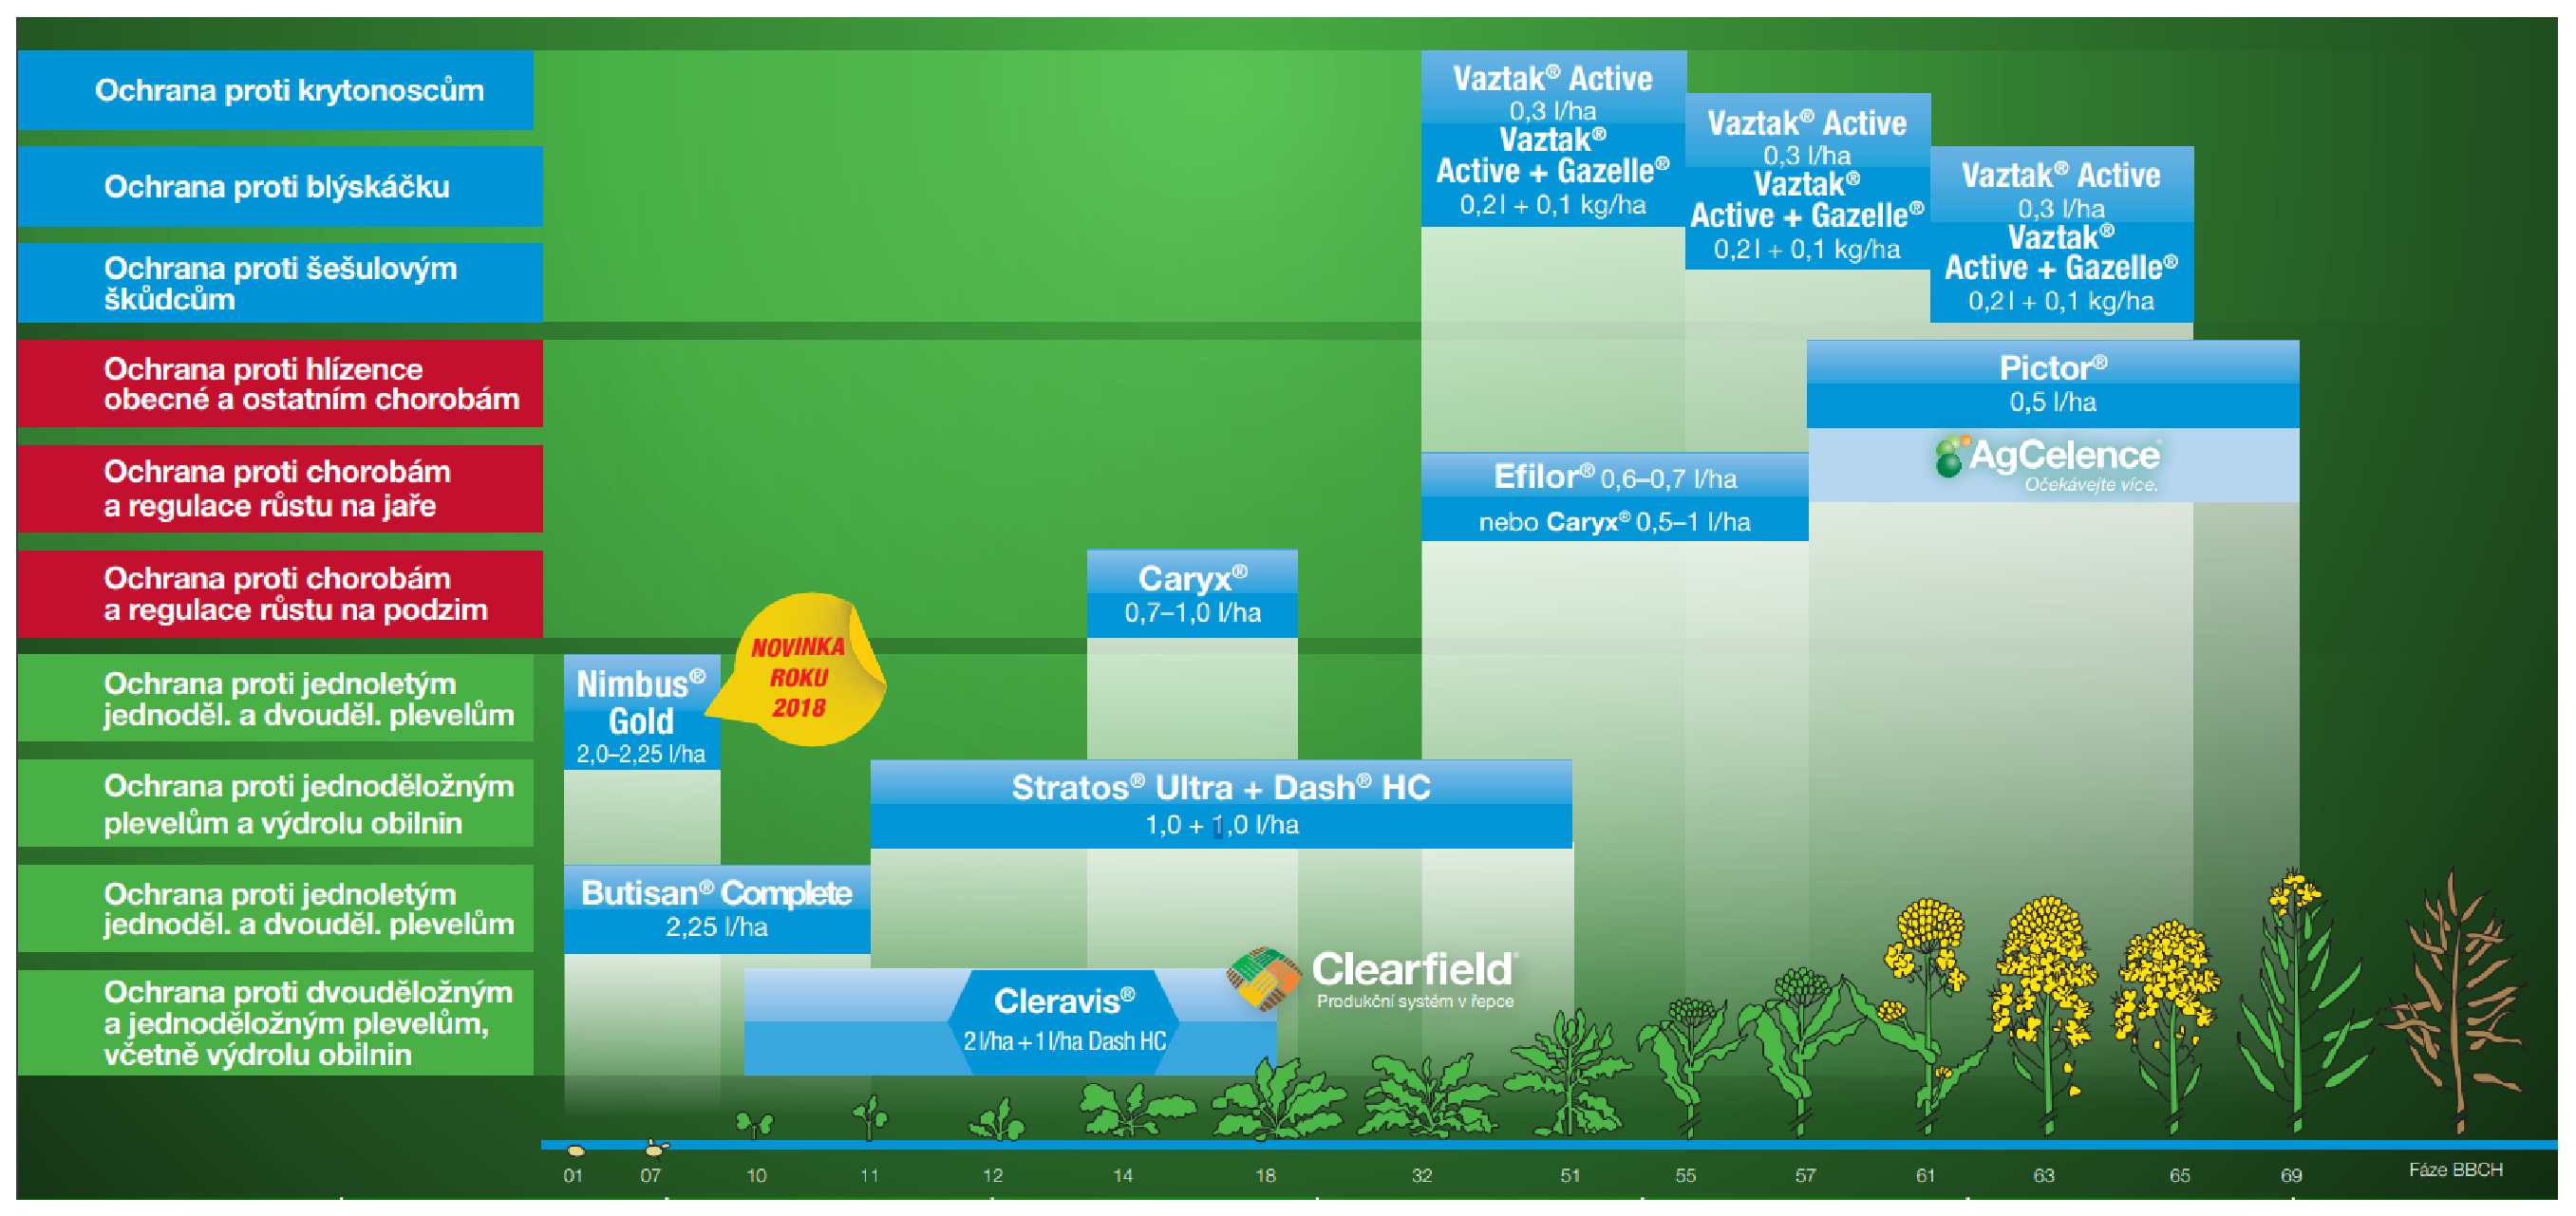
\includegraphics[width=170mm]{img/basf_postriky.eps}
\caption{Ochrana řepky proti škodlivým činitelům firmy BASF \label{basf_postriky}}
\end{figure}
Používané přípravky se dělí do několika skupin, to je důležité hlavně kvůli informaci o mísitelnosti jednotlivých přípravků.
\begin{itemize}
  \item Listová hnojiva.
  \item Fungicidy.
  \item Insekticidy.
  \item Herbicidy.
  \item Graminicidy.
\end{itemize}

\subsection{Ochrana proti krytonoscům, blýskáčku a šešulovým škůdcům}
Použitý přípravek se nazývá Vaztak Active\footnote{Vaztak je přípravek německého výrobce BASF: \\\url{\detokenize{
https://www.agro.basf.cz/agroportal/cz/cs/crop_protection/vyhled_v_n__p__pravk__podle_parametr_/product_details_24923.html
}}.}.
\begin{itemize}
  \item Spotřeba 0,3l/ha. * 3 za každé období postřiku.
  \item Doporučené množství vody 200–600 l/ha (polní plodiny, zelenina), 200–1000 l/ha (prostorové plodiny) 
  \item Kategorie Insekticidy.
  \item Mísit lze se vším.
  \item Cena 815 bez DPH za litr.
\end{itemize}

\subsection{Ochrana proti hlízence obecné a ostatním chorobám}
Použitý přípravek se nazývá Pictor\footnote{Pictor je přípravek německého výrobce BASF: \\\url{\detokenize{
https://www.agro.basf.cz/agroportal/cz/cs/crop_protection/vyhled_v_n__p__pravk__podle_parametr_/product_details_1396.html
}}.}.
\begin{itemize}
  \item Spotřeba 0,5l/ha.
  \item Doporučené množství vody 200-400l/ha.
  \item Kategorie Fungicidy.
  \item Mísit lze se vším.
  \item Cena 3280 bez DPH za litr.
\end{itemize}

\subsection{Ochrana proti chorobám a regulace růstu na jaře}
Použitý přípravek se nazývá Efilor\footnote{Efilor je přípravek německého výrobce BASF: \\\url{\detokenize{
https://www.agro.basf.cz/agroportal/cz/cs/crop_protection/vyhled_v_n__p__pravk__podle_parametr_/product_details_72192.html
}}.}.
\begin{itemize}
  \item Spotřeba 0,6l/ha.
  \item Doporučené množství vody 150-400l/ha.
  \item Kategorie Fungicidy.
  \item Mísit nelze pouze pýrohubné dávky u Graminicidů.
  \item Cena 1399 bez DPH za litr.
\end{itemize}
Efilor zajišťuje vynikající ochranu proti houbovým chorobám a kompaktní porosty s ideální architekturou, které díky tomu rovnoměrně kvetou a dozrávají.

\subsection{Ochrana proti chorobám a regulace růstu na podzim}
Použitý přípravek se nazývá Caryx\footnote{Caryx je přípravek německého výrobce BASF: \\\url{\detokenize{
https://www.agro.basf.cz/agroportal/cz/cs/crop_protection/vyhled_v_n__p__pravk__podle_parametr_/product_details_1446.html
}}.}.
\begin{itemize}
  \item Spotřeba 0,75-1l/ha.
  \item Doporučené množství vody 150-400l/ha.
  \item Kategorie Fungicidy.
  \item Mísit nelze pouze pýrohubné dávky u Graminicidů.
  \item Cena 1009 bez DPH za litr.
\end{itemize}

\subsection{Ochrana proti jednoletým jednoděl. a dvouděl. plevelům}
První možný přípravek se nazývá Butisan Complete\footnote{Butisan Complete je přípravek německého výrobce BASF: \\\url{\detokenize{
https://www.agro.basf.cz/agroportal/cz/cs/crop_protection/vyhled_v_n__p__pravk__podle_parametr_/product_details_85632.html
}}.}.
\begin{itemize}
  \item Spotřeba 2-2,25l/ha.
  \item Doporučené množství vody 100-400l/ha.
  \item Kategorie Herbicidy.
  \item Mísit lze se vším.
  \item Cena 1016 bez DPH za litr.
\end{itemize}

Druhý možný přípravek se nazývá Nimbus Gold\footnote{Nimbus Gold je přípravek německého výrobce BASF: \\\url{\detokenize{
https://www.agro.basf.cz/agroportal/cz/cs/crop_protection/vyhled_v_n__p__pravk__podle_parametr_/product_details_99459.html
}}.}.
\begin{itemize}
  \item Spotřeba 2-2,25l/ha.
  \item Doporučené množství vody 100-400l/ha.
  \item Kategorie Herbicidy.
  \item Mísit lze se vším.
  \item Cena 919 bez DPH za litr.
\end{itemize}

\subsection{Ochrana proti jednoděložným plevelům a výdrolu obilnin}
Použitý přípravek se nazývá Stratos Ultra\footnote{Stratos Ultra je přípravek německého výrobce BASF: \\\url{\detokenize{
https://www.agro.basf.cz/agroportal/cz/cs/crop_protection/vyhled_v_n__p__pravk__podle_parametr_/product_details_1429.html
}}.}.
\begin{itemize}
  \item Spotřeba 1l/ha.
  \item Doporučené množství vody 200-300l/ha.
  \item Kategorie Herbicidy.
  \item Mísit nelze s listovým hnojivem Solubor.
\end{itemize}
Pomocný přípravek se nazývá Dash HC\footnote{Dash HC je přípravek německého výrobce BASF: \\\url{\detokenize{
https://www.agro.basf.cz/agroportal/cz/cs/crop_protection/vyhled_v_n__p__pravk__podle_parametr_/product_details_1441.html
}}.}.
\begin{itemize}
  \item Spotřeba 1l/ha.
  \item Doporučené množství vody 300l/ha.
\end{itemize}
Cena za 10l přípravku Stratos Ultra a 10l přípravku Dash HC je 6990 bez DPH.

\subsection{Ochrana proti dvouděložným a jednoděložnám plevelům, včetně výdrolu obilnin}
Použitý přípravek se nazývá Cleravis\footnote{Cleravis je přípravek německého výrobce BASF: \\\url{\detokenize{
https://www.agro.basf.cz/agroportal/cz/cs/crop_protection/vyhled_v_n__p__pravk__podle_parametr_/product_details_55941.html
}}.}.
\begin{itemize}
  \item Spotřeba 2l/ha.
  \item Doporučené množství vody 300-400l.
  \item Kategorie Herbicidy.
  \item Mísit nelze s Graminicidy.
\end{itemize}
Pomocný přípravek se nazývá Dash HC.
\begin{itemize}
  \item Spotřeba 1l/ha.
  \item Doporučené množství vody 300l/ha.
\end{itemize}
Cena za 10l přípravku Cleravis a 5l přípravku Dash HC je 11699 bez DPH.
